\documentclass[%
 reprint,
%superscriptaddress,
%groupedaddress,
%unsortedaddress,
%runinaddress,
%frontmatterverbose, 
%preprint,
%showpacs,preprintnumbers,
%nofootinbib,
%nobibnotes,
%bibnotes,
 amsmath,amssymb,
 aps,
%pra,
%prb,
%rmp,
%prstab,
%prstper,
%floatfix,
]{revtex4-2}

\usepackage{graphicx}% Include figure files
\usepackage{dcolumn}% Align table columns on decimal point
\usepackage{bm}% bold math
%\usepackage{hyperref}% add hypertext capabilities
%\usepackage[mathlines]{lineno}% Enable numbering of text and display math
%\linenumbers\relax % Commence numbering lines

%\usepackage[showframe,%Uncomment any one of the following lines to test 
%%scale=0.7, marginratio={1:1, 2:3}, ignoreall,% default settings
%%text={7in,10in},centering,
%%margin=1.5in,
%%total={6.5in,8.75in}, top=1.2in, left=0.9in, includefoot,
%%height=10in,a5paper,hmargin={3cm,0.8in},
%]{geometry}

%% Added by me: this forces the table caption to be on top.
\usepackage{lipsum}
\usepackage{hyperref}
\usepackage{floatrow}
\usepackage{gensymb}
\usepackage[thinc]{esdiff}
\floatsetup[table]{capposition=top}


\begin{document}

\preprint{APS/123-QED}

\title{Generation and Analysis of Gas Particle Velocities from Maxwell-Boltzmann Distributions}% Force line breaks with \\

\author{Neema Rafizadeh}
\altaffiliation[Email: ]{ rafizadehn@ku.edu}
\affiliation{%
Department of Physics and Astronomy, University of Kansas, Lawrence, KS, 66045, USA\\
% This line break forced with \textbackslash\textbackslash
}%

\date{\today}
%\date{\today}% It is always \today, today,
             %  but any date may be explicitly specified

\begin{abstract}

This experiment observed the ability for an apartment tenant to decide whether to trust their landlord about the air conditioner in their unit. To determine whether their apartment was actually a different temperature than the temperature outside, individual gas particles were sampled for their velocities and collected into a distribution. This was then compared to the null hypothesis and a statistical power analysis was performed. The number of particles was found to be less than 250 particles sampled to reach an 80\% confidence level in the ability to resolve the distributions. 
\end{abstract}


%\keywords{Suggested keywords}%Use showkeys class option if keyword
                              %display desired
\maketitle

%\tableofcontents

\section{Introduction \protect\\ }

Many physical systems studied in modern physics research follow the Maxwell-Boltzmann (MiB) distribution. From the study of electron diffusion in the semi-metal graphene to the modeling of photon interactions between a laser and a solid in photonics, the M-B distribution has proven to have great utility in explaining observed physical phenomena. The distrubtion has more fundamental roots in its derivation from the first principles of mass, temperature, and velocity of gas particles, though how well can M-B curves truly be distinguished from one another?  

If there exists a room that has an unknown temperature, the M-B distribution can be used to experimentally determine its temperature by sampling particles from the gas in equilibrium in the room. The process of removing individual gas particles from a room and measuring its velocity by hand turns out to be quite arduous and taxing, thus determining the fewest number of particles that need to be sampled before a temperature can be determined is useful to know.

Take, for example, an apartment resident is told that their unit has an air conditioner set at 310 K while the temperature outside the building is 275 K. If the resident thinks their landlord is lying, they might want to determine if the air conditioner exists without access to the conditioner itself. If they are able to measure the velocities of individual gas particles in the room, they can tell whether the conditioner is functioning by sampling the M-B distribution. The questions that they must consider become: \textit{are the possible temperatures too close to be distinguished experimentally?} and \textit{how many particles do we need to measure before we can tell?}

Through probability statistics and power analysis, these questions can be answered and save people from countless hours of measuring velocities of gas particles by hand. Maybe this isn't a real problem. Oh well. Onward anyway\dots \textit{for science}.

\section{Hypotheses of Different Temperature Gases}

The M-B distribution is derived from basic physics principles based on some assumptions, namely that the gas particles are non-interacting, non-relativstic, and in thermal equilibrium. If this is the case, then the probability that you find a particle with a particular velocity is given by,
\[
	f(m, v, T) = \left( \frac{m}{2\pi k T} \right)^{1/2}4\pi v^2 e^{-\frac{mv^2}{2kT}},
\]
where $m$ represents the molecular mass of the particles and $T$ represents the equilibrium temperature of the gas. Two examples of this probability distribution are plotted in Fig. 1 with temperatures 100 K and 1000 K. 

\begin{figure}[h]
	\caption{Probability density for gas particle velocity at differing temperatures, 100 k and 1000 K. Values taken for a gas with an 85 amu molecular mass. }
	\centering
	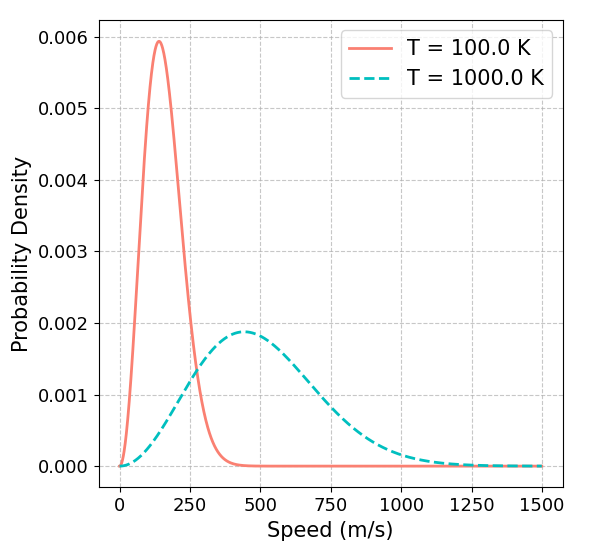
\includegraphics[scale=0.51]{hypothesis1.png}
\end{figure}

Note this is a probability \textit{density}, not a direct probability. Thus, the probability can be calculated through integration over a range of particle velocity. This means that the probability to find a particle at one particular velocity is 0 m/s as the integral will have the same two bounds. Because of this, many statisticians plot cumulative density functions which represent the area under the curve of the probability density function up to a given value of velocity.


\section{Code and Experimental Simulation}

The plots in Fig. 1 are idealized curves that are plotted directly from the M-B distribution equation. To simulate a real experiment sampling gas particles, a random number generator is used in conjunction with the M-B equation and plotted as a histogram shown in Fig. 2.

\begin{figure}[h]
\caption{Histogram of particle velocities taken at a N = 1000 sample size. Values taken for a gas with an 85 amu molecular mass.}
\centering
	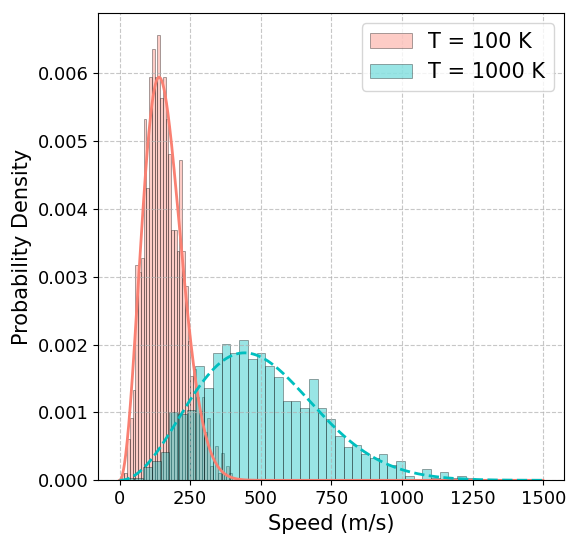
\includegraphics[scale=0.51]{code1}
\end{figure}

As seen in the Fig. 2, the randomly generated velecity values closely resemble the idealized curves from before. See Appendix B to reference how the randomly generated velocities fit better at high sample size. The temperatures shown in Figs 1. and 2. were chosen to be 100 K and 1000 K for demonstration, but this does not help the tenant in the apartment on the hunt for their elusive air conditioner. The temperatures used in the experiment are 275 K, which represents the null hyposthesis (H$_0$), and 320 K, which represents our hypothesis we are testing against the null (H$_1$).

With temperatures so close together in value, it may not be as obvious to resolve the curves as it is with the 100 K and 1000 K curves. See Appendix C for a graphical representation of the 275 K and 320 K histograms next to one another. Instead of resolving our curves graphically, we will use a statistical power analysis to differentiate between the data we collect and the data from the null hypothesis. Through analysis of our type II errors (referred to as the value $\beta$), we can determine how often our data indicates the null hypothesis when it is in fact the higher temperature, and then calculate our statistical power ($1-\beta$) from that. The statistical power is essentially the reverse of the type II error, it tells us how often we reject the null hypothesis when we should, in fact, reject it. The higher the statistical power, the easier it is to distinguish data from the two temperatures, and thus the easier it will be for the apartment tenant to determine whether his landlord is juking him with his air conditioner. 

\section{Results and Analysis}

The results of this method are shown in Fig. 3 for 320 K, but also for other temperatures in the range of 290-330 K.

\begin{figure}[h]
	\caption{Statistical power plotted as a function of sample size. Statistical power is the ability to resolve the positive hypothesis (H$_1$) to the null hypothesis (H$_0$). }
	\centering
	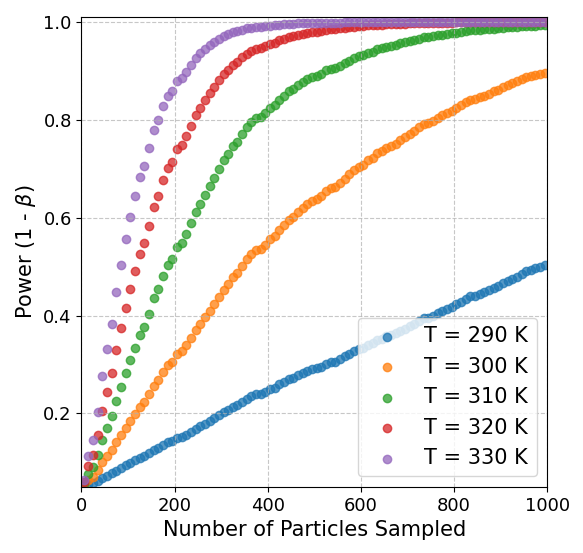
\includegraphics[scale=0.51]{results1.png}
\end{figure}

The different temperatures in Fig. 3 show the difference in statistical power per sample size in comparison to the other temperatures. Statisticians regard 0.8 to be a statistical power significant enough to consider two distributions resolvable, and as the temperature increaes, it reaches that confidence level in much fewer number of sampled particles. Since the apartment tenant is trying to resolve a temperature of 320 K, they would need to sample roughly 250 particles before reaching the 80\% confidence level.

\section{Conclusion}
The temperature of 320 K is far enough away from the temperature outside of the apartment (275 K) that the tenant of the apartment will be able to tell whether or not the landlord is lying to them at a 80\% confidence level from less than 300 particles measured. Through the use of statistical power analysis, two distributions were able to be resolved from one another. 

Not sure what else to write. I will think of something. I am so sorry you had to read this, its very boring. I had no better ideas for the project. This seemed like the easiest thing to do haha.

filling space for formatting: \lipsum[1-2]

\acknowledgements

I would like to thank Prof. Chris Rogan for his continued support in the course. I would also like to apologize to the student who was assigned to me for peer review.

\appendix
\section{Raw Data}

All python scripts and data generated are contained in \href{https://github.com/rafizadehn/PHSX815_Project1}{\textcolor{blue}{Neema Rafizadeh's GitHub repository for this project.}}

\section{Histogram of Particle Velocities at Large Sample Size}

\begin{figure}[H]
	\caption{Histogram of randomly generated particles in a Maxwell-Boltzmann distribution. Number of particles generated is at N = 100,000 particles ($10^5$).}
	\centering
	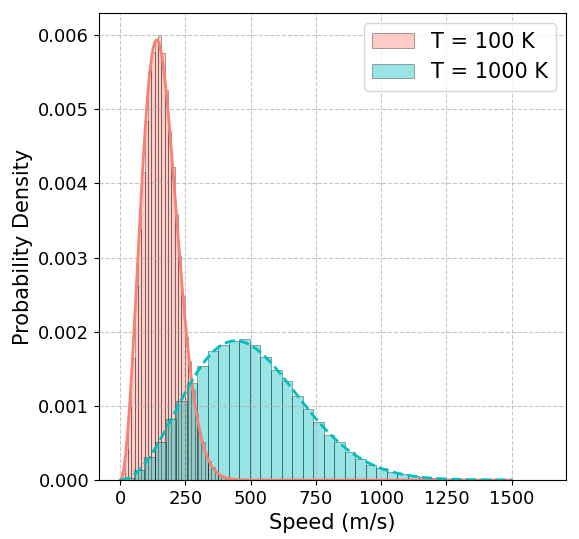
\includegraphics[scale=0.5]{appendix1.png}
\end{figure}

\section{Histogram of Particle Velocities at Scenario's Temperatures}

\begin{figure}[H]
	\caption{Probability density for gas particle velocity at differing temperatures, 275 k and 320 K. Values taken for a gas with an 85 amu molecular mass. }	
	\centering
	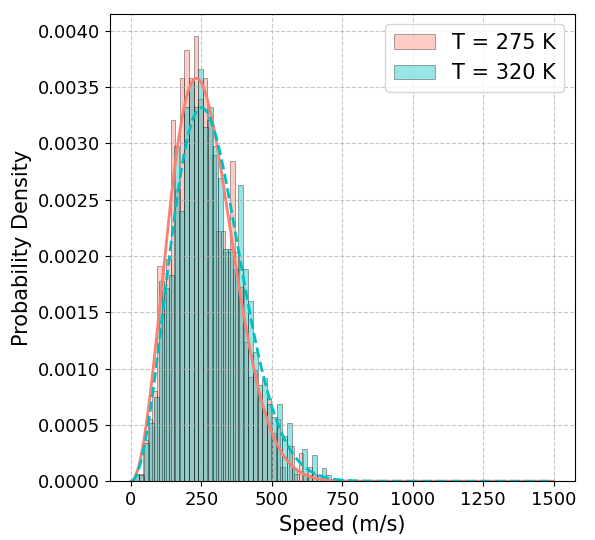
\includegraphics[scale=0.5]{appendix2.png}
\end{figure}

% The \nocite command causes all entries in a bibliography to be printed out
% whether or not they are actually referenced in the text. This is appropriate
% for the sample file to show the different styles of references, but authors
% most likely will not want to use it.
\nocite{*}

\bibliography{report_template}% Produces the bibliography via BibTeX.

\end{document}

%
% ****** End of file apssamp.tex ******
